\documentclass[12pt,fleqn,answers]{exam}
\usepackage{amssymb}
\usepackage[intlimits]{amsmath}
\usepackage{epsfig}
\usepackage{upgreek}
\usepackage[super]{nth}
\usepackage[colorlinks=true,linkcolor=black,anchorcolor=black,citecolor=black,filecolor=black,menucolor=black,runcolor=black,urlcolor=black]{hyperref}
\usepackage[letterpaper, margin=0.75in]{geometry}
\addpoints
\boxedpoints
\pointsinmargin
\pointname{pts}
\usepackage{tikz}
\usepackage{tkz-euclide}
\usetikzlibrary{shapes.geometric}
\usetikzlibrary{calc}
\usepackage[final]{microtype}
\frenchspacing
\usepackage[american]{babel}
\usepackage[T1]{fontenc}
\usepackage[]{fourier}

\usepackage{isomath}
\usepackage{upgreek,amsmath}
\usepackage{graphicx}

\newcommand{\dotprod}{\, {\scriptzcriptztyle\stackrel{\bullet}{{}}}\,}

\newcommand{\reals}{\mathbf{R}}
\newcommand{\lub}{\mathrm{lub}} 
\newcommand{\glb}{\mathrm{glb}} 
\newcommand{\complex}{\mathbf{C}}
\newcommand{\dom}{\mbox{dom}}
\newcommand{\range}{\mbox{range}}
\newcommand{\cover}{{\mathcal C}}
\newcommand{\integers}{\mathbf{Z}}
\newcommand{\vi}{\, \mathbf{i}}
\newcommand{\vj}{\, \mathbf{j}}
\newcommand{\vk}{\, \mathbf{k}}
\newcommand{\bi}{\, \mathbf{i}}
\newcommand{\bj}{\, \mathbf{j}}
\newcommand{\bk}{\, \mathbf{k}}
\DeclareMathOperator{\Arg}{\mathrm{Arg}}
\DeclareMathOperator{\Ln}{\mathrm{Ln}}
\newcommand{\imag}{\, \mathrm{i}}
\newcommand{\erf}{\mathrm{erf}}
\newcommand{\e}{\mathrm{e}}

\usepackage{graphicx}
\usepackage{color}
%\shadedsolutions
%\definecolor{SolutionColor}{rgb}{1,0.72,0.46} %{0.8,0.9,1}
\newcommand\AM{\textsc{am}}
\newcommand\PM{\textsc{pm}}


     
\newcommand{\quiz}{23}
\newcommand{\term}{Fall}
\newcommand{\due}{Tuesday 21 November 13:20}
\newcommand{\class}{MATH 202, Fall \the\year}
\begin{document}
\large
\noindent\makebox[3.0truein][l]{\textbf{\class}}
\textbf{Name:} \hrulefill \\
\noindent \makebox[3.0truein][l]{\textbf{In class work  \quiz}}
\textbf{Row and Seat}:\hrulefill\\



\noindent  In class work  \textbf{\quiz}  has questions \textbf{1} 
through  \textbf{\numquestions} \/ with a total of 
\textbf{\numpoints\/} points. Turn in your work at the end of class 
\emph{on paper}. This assignment is due at \emph{\due}.

\vspace{0.1in}

\noindent \emph{“Piglet noticed that even though he had a very small heart, 
it could hold a rather large amount of gratitude.”}
 \phantom{xxx} \hfill {\sc   A. A. Milne}


\begin{questions} 
    
    \question Consider the parametrically defined curve $\mathcal{C} = \displaystyle
    \begin{cases} x =  \frac{t}{1+t^2}, \\ y = \frac{2t^2}{1+ t^2} \end{cases},  
    -\infty < t < \infty$.


    \begin{parts}

    \part [1] Use Desmos to draw this curve. Reproduce the curve as best you can 
    on here:

    \begin{solution}[2.5in]

    Appearances are deceiving, but the curve $\mathcal{C}$ looks like an ellipse. 
    \vspace{0.1in}
    \begin{center}
    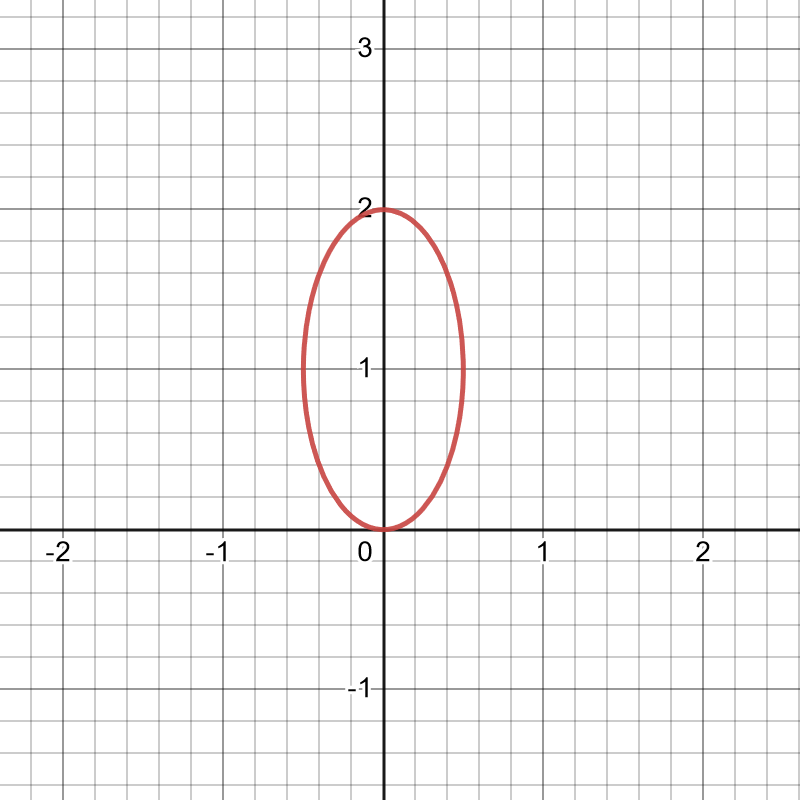
\includegraphics[scale=0.2]{desmos-graph(69).png}
    \end{center}

    \end{solution}


    \part [1] Is the point $(x=0, y=2)$ on the curve?  The picture might indicate
    that it is, but is it really? To decide, you'll need to solve the equations
    \begin{equation*}
        0 = \frac{t}{1+t^2} , \,\, 2 = \frac{2t^2}{1+ t^2}.
    \end{equation*}
    \begin{solution}%[2.5in]
     No, the point $(x=0, y=2)$ on not on the curve $\mathcal{C}$. To prove this, we need to solve
     the equations
     \begin{equation*}
        \left[ 0 = \frac{t}{1+t^2} ,  2 = \frac{2t^2}{1+ t^2} \right] 
        = \left[ 0 = t, 2 + 2t^2 = 2 t^2 \right]
        = \left[ 0 = t, 2  = 0 \right] 
    \end{equation*}
    The solution set is empty, so $(x=0, y=2)$ on not on the curve $\mathcal{C}$.
    
    \textbf{Notice} We're solving two equations for one unknown.
    We need to find a common solution for both equations. The second
    equation has no solution, so the solution set is empty.
    
    \quad Arguably, $t = \infty$ is a solution of the equations $\left[ 0 = \frac{t}{1+t^2} ,  2 = \frac{2t^2}{1+ t^2} \right]$.
    Indeed $\displaystyle \lim_{t \to \infty} \frac{t}{1+t^2} = 0$ and $\displaystyle \lim_{t \to \infty} \frac{2t^2}{1+ t^2} = 2$. 
    So it's tempting to say that $(x=0, y=2) \in \mathcal{C}$, but 
    we'd need to extend the domain to make that true.
  \end{solution}

    \newpage
    
    \part [1] Solve $\displaystyle \frac{\mathrm{d} y} {\mathrm{d} t} = 0$
    and $\displaystyle \frac{\mathrm{d} x} {\mathrm{d} t} \neq  0$.  Each solution
    will give a point on the curve with a horizontal tangent line. 
   


    \begin{solution}[3.5in]
    \begin{equation}
        \left[0 = \frac{\mathrm{d} y} {\mathrm{d} t} \right] = 
        \left[0 = \frac{4 t}{1+t^2}\right] = [t=0]
     \end{equation}

  
A calculation shows that when $t=0$, we have $\left. \frac{\mathrm{d} x} {\mathrm{d} t} \right |_{t=0} = 1$. So 
the only HT happens when $t=0$.  And that makes $x=0$ and $y=0$.

\quad The picture might make us think that there is a HT 
at the point $(x=0, y=2)$. But $(x=0, y=2) \notin \mathcal{C}$, 
so I would say that the curve doesn't have an HT at $(x=0, y=2)$. 
Others could quibble with that--to settle this, we'd need a 
precise definition of HT.

    \end{solution}

    

  \part [1] Substitute $\begin{cases} x =  \frac{t}{1+t^2} \\ y = \frac{2t^2}{1+ t^2} 
\end{cases}$ into $4 x^2 + y^2 - 2 y = 0$. Explain why that shows that the curve 
$\mathcal{C}$ is a \emph{portion} of an ellipse, but not the entire ellipse.

    \begin{solution}[3.5in] Let $x = \frac{t}{1+t^2}$ and let $y = \frac{2t^2}{1+ t^2} $
    into $4 x^2 + y^2 - 2 y = 0$ gives
    \begin{equation}
    4  \left(\frac{t}{1+t^2}^2 \right)^2  +  \left(\frac{2t^2}{1+ t^2} \right) - 2  \frac{2t^2}{1+ t^2} = 0.
    \end{equation}
  We've shown that if $x =  \frac{t}{1+t^2}$ and $y = \frac{2t^2}{1+ t^2} $, then $4 x^2 + y^2 - 2 y = 0$.
    
\quad We did not show that if $4 x^2 + y^2 - 2 y = 0$, there is a number $t$ such that $\begin{cases} x =  \frac{t}{1+t^2} \\ y = \frac{2t^2}{1+ t^2} 
\end{cases}$. And it's a good thing we didn't prove it because it is false.  
It's false because $(x=0,y=2)$ is a point on 
the graph of  $4 x^2 + y^2 - 2 y = 0$, but  $(x=0,y=2) \notin \mathcal{C}$.
 
\quad Actually the curve $\mathcal{C}$ is the ellipse $4 x^2 + y^2 - 2 y = 0$
with exactly one point missing.  To append this missing point, we could define
\begin{equation*}
  \mathcal{C}^\star = 
  \begin{cases} x =  \begin{cases} \frac{t}{1+t^2} & t \neq \infty \\
                                  0 & t = \infty 
                     \end{cases} \\ 
              y = \begin{cases}  \frac{2t^2}{1+ t^2} & t \neq \infty \\
                                  2 & t = \infty
              \end{cases}
              \end{cases},  
  -\infty < t \leq \infty.
\end{equation*}

\quad Finally, I know what you are thinking.  How did I eliminate the parameter $t$ from  $\begin{cases} x =  \frac{t}{1+t^2} \\ y = \frac{2t^2}{1+ t^2} 
\end{cases}$ to discover $4 x^2 + y^2 - 2 y = 0$?  There is a beautify algorithm for doing this--it involves the polynomial
resultant. Ending in the 1950s, I think, such things were taught in a class that was generally called the Theory of Equations.


\end{solution}

\end{parts}
\end{questions}
    
\end{document}
